\begin{figure}[h]
    \noindent\makebox[\textwidth]{
    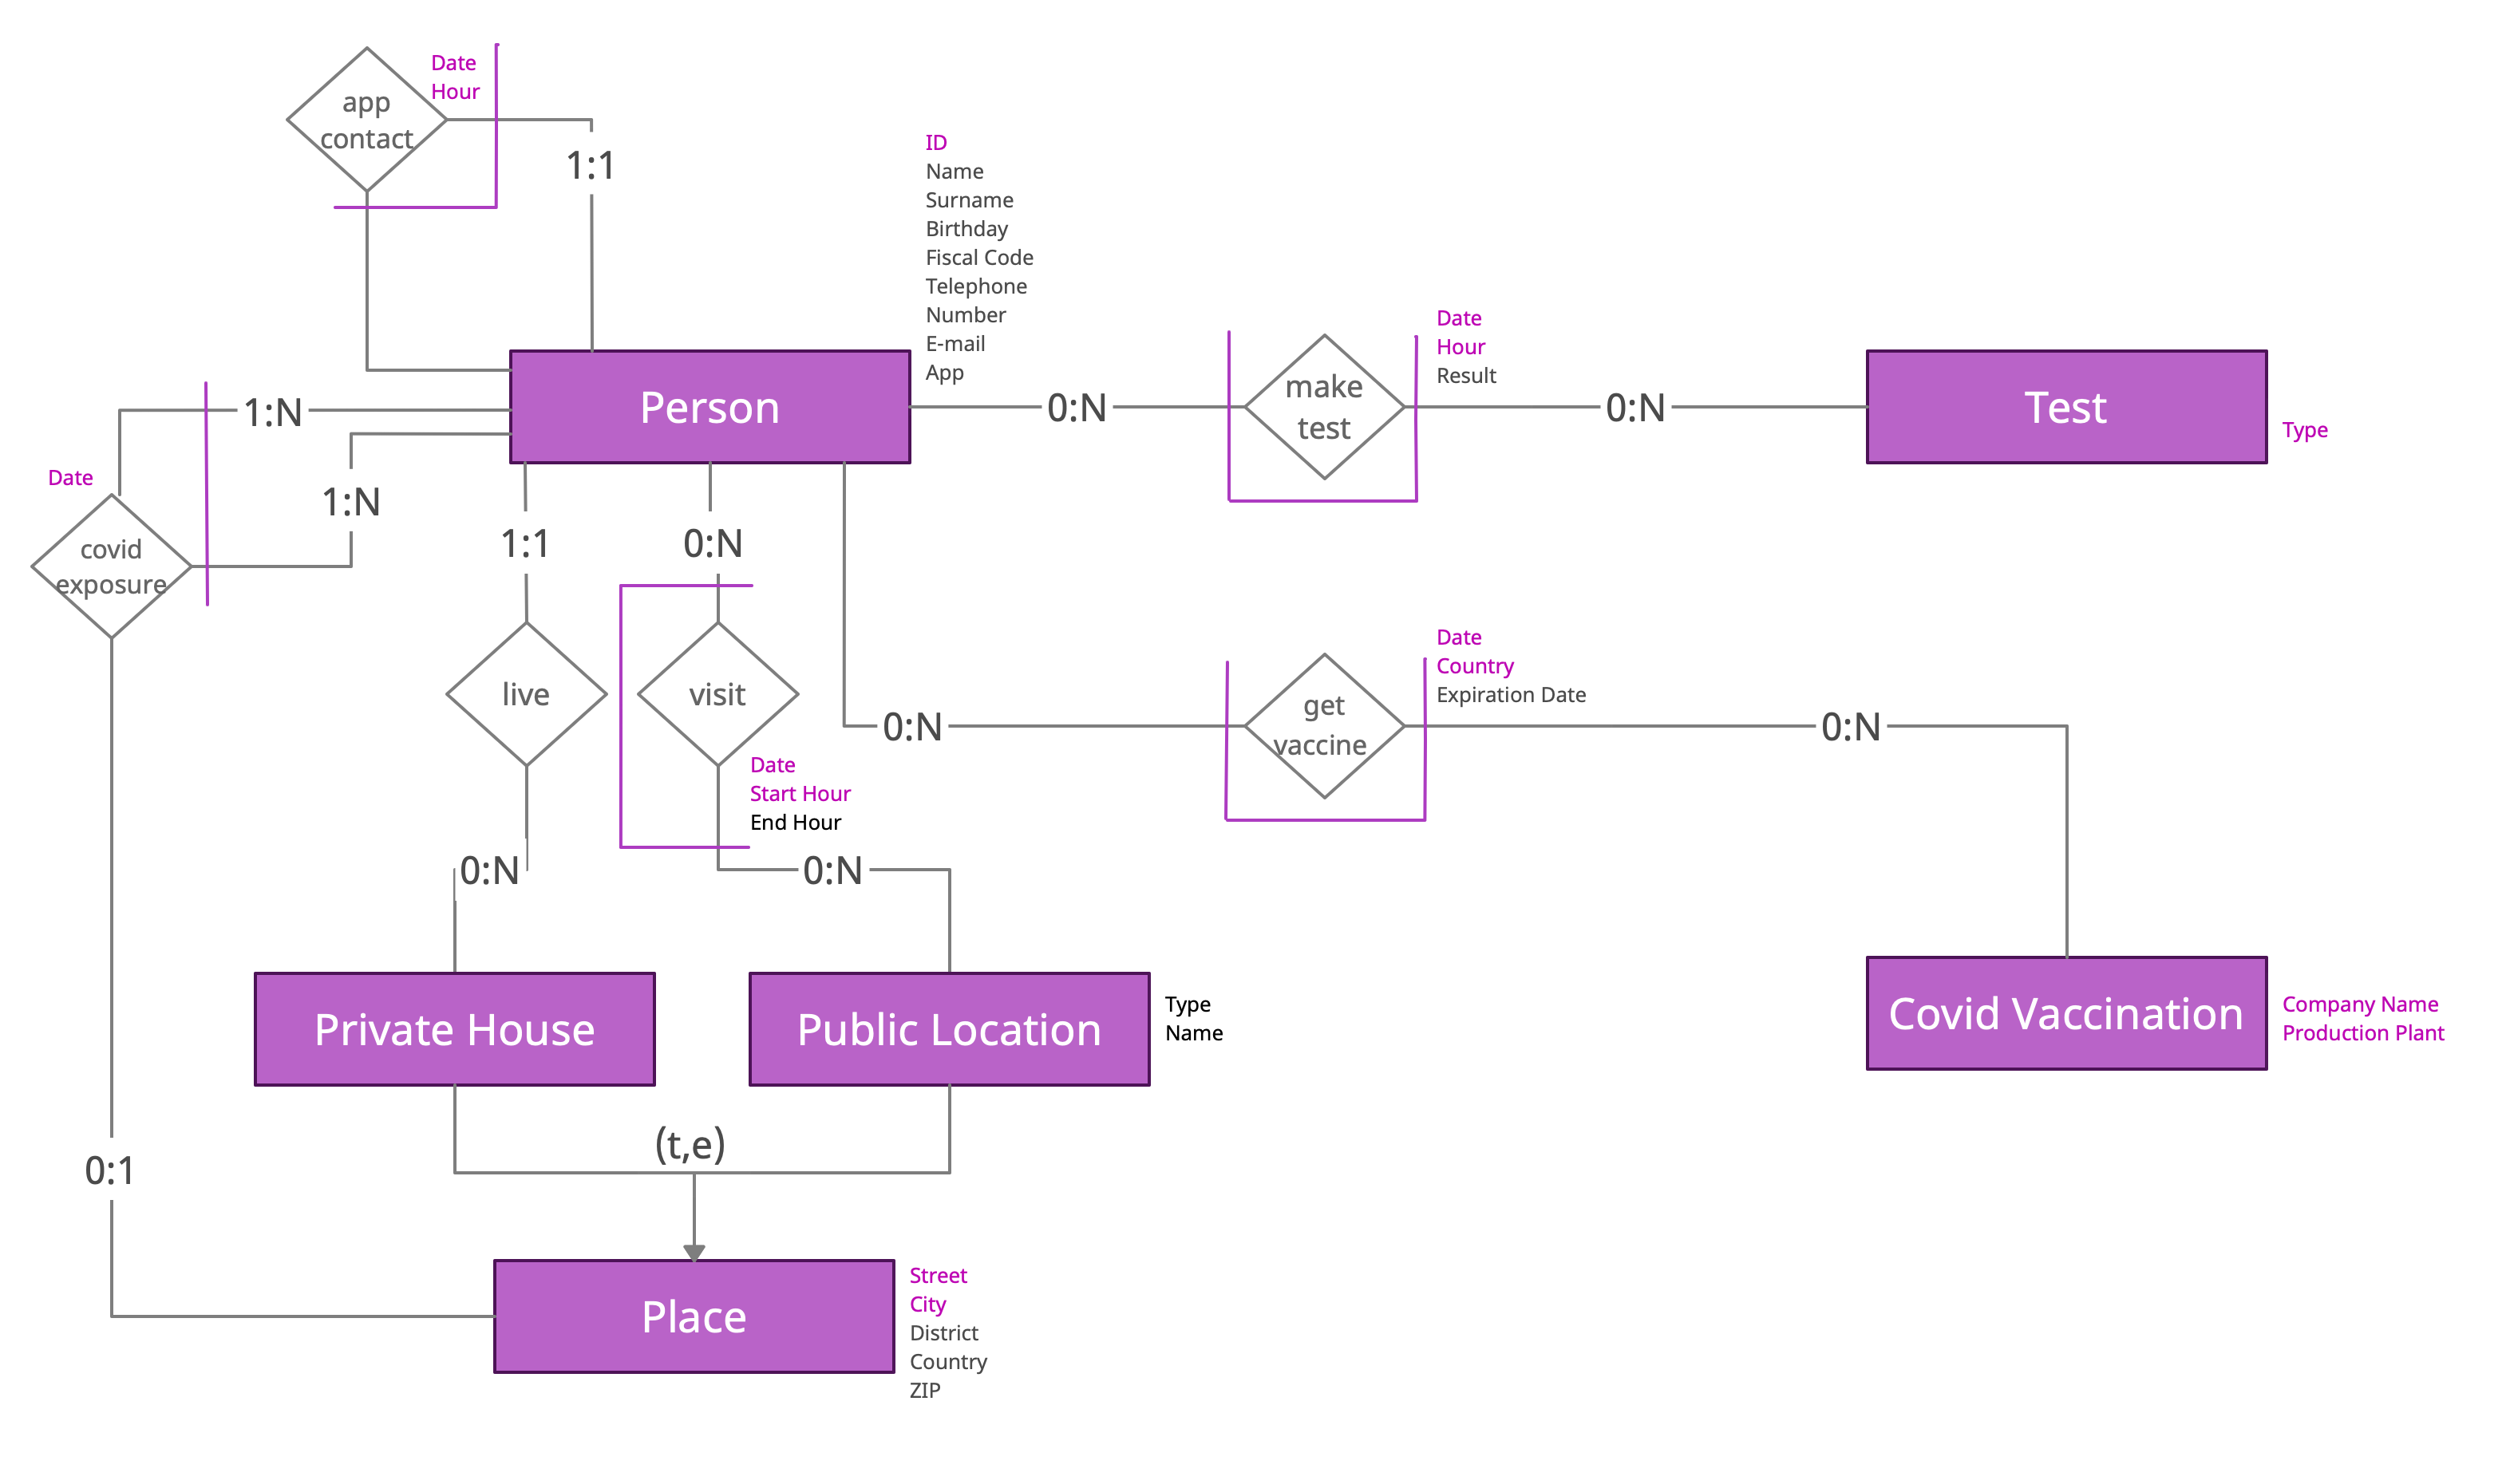
\includegraphics[width=0.8\paperwidth]{images/ImmunoPoli-ER.jpg}
}
\caption{\textit{Entity Relationship model}}
\end{figure}

\subsection{Entities}
\begin{itemize}
    \item \textbf{Person} entity is identified by his ID. 
    \item \textbf{Place} represents an abstraction for the objects that have an address.
    \item \textbf{Private house} hosts either a group of flatmates or a family.
    \item \textbf{Public place} represents indoor places accessible showing Covid certification and a valid pass.
    \item \textbf{Covid Vaccination} provides an abstraction for vaccine. It is identified through its firm name and the production plant from where it comes.
\end{itemize}

\newpage
\subsection{Relationships}
\begin{itemize}
    \item The \textit{infect} relationship represents a \textbf{possible viral infection}. Once a positive test is inserted into the database, the system triggers a command to easily find all the people at risk of contagion and notify them. People are obliged to make a swab, and in case of a negative result, the relationship is deleted.
    \item The \textit{live} relationship binds a person with where he resides.
    \item The \textit{visit} relationship involves all the public places where it is more likely that personal information is collected. It serves both realism and simplicity purposes because we don't need to take care of outdoor spots.
    \item The \textit{app contact} relationship gathers all contacts detected by any tracking system that supports localization and application installations, regardless of its type.
\end{itemize}